\documentclass[conference, final]{IEEEtran}
%\documentclass[conference]{IEEEtran}
\IEEEoverridecommandlockouts
% The preceding line is only needed to identify funding in the first footnote. If that is unneeded, please comment it out.
\usepackage{cite}
\usepackage{amsmath,amssymb,amsfonts}
\usepackage{algorithmic}
\usepackage{graphicx}
\usepackage{textcomp}
\usepackage{xcolor}
\usepackage{multirow}
\usepackage{comment}
\usepackage{booktabs}

\usepackage[bordercolor=gray!20,backgroundcolor=red!10,linecolor=red!50,textsize=scriptsize,textwidth=0.51in,obeyFinal]{todonotes}
\setlength{\marginparwidth}{0.51in}
\setlength{\marginparsep}{0.10in}
\usepackage{soul}
\def\BibTeX{{\rm B\kern-.05em{\sc i\kern-.025em b}\kern-.08em
    T\kern-.1667em\lower.7ex\hbox{E}\kern-.125emX}}
\bibliographystyle{ieeetr}

% ======================================
% trying to save space
\usepackage[compact]{titlesec}
\titlespacing{\section}{0pt}{0pt}{0pt}
\AtBeginDocument{
  \setlength\abovedisplayskip{0pt}
  \setlength\belowdisplayskip{0pt}}
\setlength{\textfloatsep}{2pt plus 0pt minus 0pt}
\setlength{\floatsep}{2pt plus 0pt minus 0pt}
\setlength{\intextsep}{2pt plus 0pt minus 0pt}
% ======================================  

%\renewcommand{\textcolor}[2]{#2}
\newcommand{\red}[1]{\textcolor{red}{#1}}
\newcommand{\green}[1]{\textcolor{green}{#1}}
\newcommand{\az}[1]{\todo[backgroundcolor=blue!10,linecolor=blue!50]{\textbf{Zaher:} #1}}


\begin{document}
\setstcolor{blue}
\title{Drones with Networking and Machine Learning for Smart City Applications: A Review\\
%{\footnotesize \textsuperscript{*}Note: Sub-titles are not captured in Xplore and
%should not be used}
\thanks{Identify applicable funding agency here. If none, delete this.}
}

\author{\IEEEauthorblockN{Masud Ahmed\textsuperscript{*}, Naima Khan, Abu Zaher Md Faridee, Nirmalya Roy}
\IEEEauthorblockA{\textit{dept. Information Systems} \\
\textit{University of Maryland Baltimore County}\\
Baltimore, USA \\
%*mahmed10@umbc.edu
}
}

\maketitle

\begin{abstract}
Unmanned Aerial Vehicle\textcolor{red}{s}, alternatively known as drone\textcolor{red}{s}, operate without any pilot on board. Starting with
surveillance, disaster management, infrastructure monitoring, drones provide unparalleled opportunities to improve our daily life with large scale IoT (Internet of thing\textcolor{blue}{s}) based applications. Nonetheless, the drone systems are facing significant limitations \textcolor{red}{in a number of areas, such as} autonomous operation, \textcolor{red}{sustaining} longer flight duration, large\textcolor{red}{-scale} data collection,
% on a single platform, 
obstacle avoidance, reliable real-time application \textcolor{red}{etc.} In this review paper, we first summarize a few research works that have proposed solutions to these constraints. We then discuss recent machine learning-based drone applications that can increase our working efficiency in numerous sectors. After that, we analyze different communication protocols and sensors that are being used with drones. We also present several drone-based challenges and datasets that may help the upcoming researchers in this field. Finally, we conclude our review by discussing the applications of drones in the current COVID-19 situation and the effects of the pandemic on the overall drone industry.

\end{abstract}

\begin{IEEEkeywords}
UAV, ummanned aerial vehicle, drone, inspection, tracking, autonomous navigation, safe landing, disaster management, supply chain, COVID-19.
\end{IEEEkeywords}

\section{Introduction}
\label{introductionsection}
\noindent \red{Over the last few years, we have observed a meteoric rise in the use and adoption of unmanned aerial vehicles (UAVs) and drones.} The first documented use of a drone for warfare occurred in  1849 when an unmanned balloon loaded with explosives attacked another town ~\cite{mckenna2016public}.
% After that, a generation of drones sparked in 1903 by the development of the fixed-wing aircraft. 
\textcolor{red}{
The development of fixed wing aircraft in 1903 sparked the development of a new generation of drones.}
% \todo{This line doesn't sound right}
The US army improved drones as weapons during the First World War, but those innovative drones were not deployed before the war ended in 1918. 
\red{World War II saw the first military use of drone as surveillance aircraft. The cold war between the east and the west further precipitated the development of drones as}.
% between many countries increased, enhancing the use of drones. 
many armed forces started using drones as a weapon, a reconnaissance tool, and a decoy. The progress of drone inspired both military and non-military companies to invest more in the field of drone research and development.

\textcolor{red}{Over the years,}
the drones saw exponential \textcolor{red}{development} for \textcolor{red}{regional} surveillance and supervision of remote construction projects. Rapid advancements in sensing, battery, and aeronautical technology, along with autonomous navigation methods and low-cost digital cameras have helped \textcolor{blue}{to} make the drone \textcolor{blue}{operations} more powerful, safer and \textcolor{blue}{reliable}\cite{liu2014review}. Since the early pioneering days, almost all types of active and passive sensors have been mounted on aerial systems, ranging from tethered to autonomous or manually operated \cite{sensing2015disasters, dong2013comprehensive}. With the help of these sensors, a drone can be deployed in many sectors, such as building inspection, rescue missions.
% , following an unidentified person, etc. 
In the present day, large number of organizations in different sectors are using drones to visually monitor the problems, 
find solutions, and even solve the problem based on the task\red{s}. Such systems are aimed at achieving more efficient service, inspection, and maintenance with minimal human intervention.

The drone-based \textcolor{blue}{monitoring} allows low-cost and frequent inspections \textcolor{blue}{with} high-resolution image analysis and limited human interference
% \st{, allowing for predictive maintenance} 
at reduced costs~\cite{morgenthal2014quality}. Lots of real-time problems exhibit recognizable visual characteristics that drones can \red{resolve} with RGB cameras~\cite{roy2013performance}. For example, cracks in the concrete 
% \st{of other} 
surfaces are visible by naked eyes. But it takes substantial manual effort to obtain damage information \red{around} \textcolor{blue}{large} scale areas.
\red{For example, taking pictures during manual inspection from a 40-50 feet height without costly safety gear poses serious risks of injury; maintaining precision while covering the whole are can also be challenging.}
% Additionally, \textcolor{blue}{frequent} manual inspection is not only challenging but also risky in some cases. Taking pictures \textcolor{blue}{from} a height \textcolor{blue}{of} 40 to 50 feet is dangerous because it may \textcolor{blue}{cause severe life threatening incidents.} 
% \st{be lethal if someone falls from that altitude} 
% Besides, 
% \textcolor{blue}{Maintaining precision and covering the whole area might not be possible with manual inspection.} 
% \st{important information might be left behind}.
\textcolor{blue}{However,} 
% \st{But in serval cases}, 
regular monitoring is necessary \textcolor{blue}{in several aspects of different domains, such as,} 
% \st{which can prevent several accidents, e.g.,} 
windmill turbine monitoring, building crack inspection, long bridge health investigation \textcolor{blue}{etc}. By 
% \st{supplying}
\textcolor{blue}{providing} 
% \st{experts with} 
automated feedback on 
% \st{highly}
\textcolor{blue}{most} likely 
% \st{locations}
\textcolor{blue}{region} of 
% \st{destruction}
\textcolor{blue}{interest where immediate action is needed}, we can significantly reduce the required man-hours \textcolor{blue}{for whole area inspection} and simultaneously increase the efficiency of \textcolor{blue}{resource usage}
% \st{manual detection, while reducing the human costs associated with the data inspection}. 
Besides \textcolor{blue}{of monitoring physical infrastructures,} 
% \st{building inspection}, 
drones can \textcolor{blue}{also} be used for \textcolor{blue}{other purposes, such as,} human 
% \st{suspectable} 
activity monitoring\textcolor{blue}{,}  
% \st{or}
rule-breaking vehicle tracking~\cite{ngo2019isir} \textcolor{blue}{etc}. Drones with 
% \st{other}
\textcolor{blue}{different} sensors can 
% \st{represent} 
\textcolor{blue}{provide variety of} other information \textcolor{blue}{of surroundings}, that can improve our daily livings in many ways~\cite{roy2015aarpa, pathak2015acoustic}. \textcolor{blue}{For an instance, hand-held or smartphone associated thermal cameras for detecting i}nsulation issues in 
% \st{built-up}
\textcolor{blue}{built-in} environments 
% \st{can be detected using a drone thermal camera which can save energy}
(i.e., ~\cite{khan2019detecting, khan2015demo, khan2020temporal}) \textcolor{blue}{ can be replaced by drone-based thermal camera for robust and scalable monitoring which can contribute to energy savings}. Common applications of drones in different sectors are shown in Fig~\ref{applicaitonfig}.


\begin{figure}[h!]
\centering
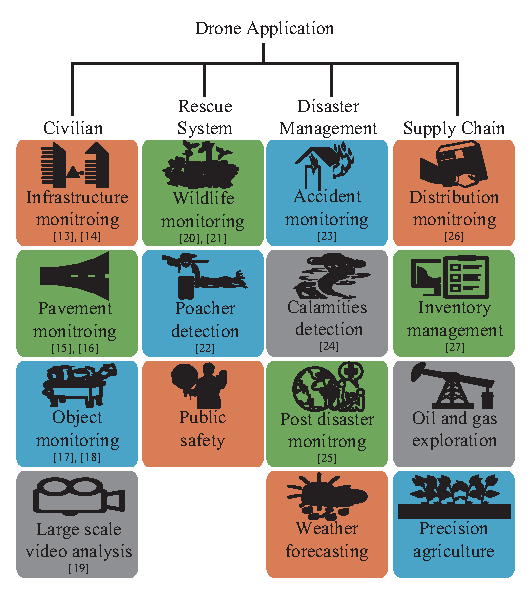
\includegraphics[width=.85\linewidth]{figure/applicaitonfig.eps}
\caption{Application of drone in different sector.}
\label{applicaitonfig}
\end{figure}
%\begin{table}[h]
\centering
\caption{Application of drones in different sector}
\begin{tabular}{|l|l|}
\hline
Category                             & \multicolumn{1}{c|}{Application}                                                                                             \\ \hline
\multirow{4}{*}{Civilian}            & Infrastructure crack detection~\cite{kucuksubasi2018transfer, kang2018autonomous}                                            \\ \cline{2-2} 
                                     & Road or pavement monitoring~\cite{wu2018coupling, fan2019real}                                                               \\ \cline{2-2} 
                                     & Object detection~\cite{li2017visual,saribas2019hybrid}                                                                       \\ \cline{2-2} 
                                     & Large scale video analysis~\cite{zhang2019dense}                                                                             \\ \hline
\multirow{2}{*}{Rescue system}       & Wildlife monitoring~\cite{mayer2019drones,brennan2019drones}                                                                 \\ \cline{2-2} 
                                     & Poacher detector~\cite{bondi2018spot}                                                                                        \\ \hline
\multirow{3}{*}{Disaster management} & \begin{tabular}[c]{@{}l@{}}Autonomous system able to explain\\ accident situations~\cite{garcia2018explainable}\end{tabular} \\ \cline{2-2} 
                                     & \begin{tabular}[c]{@{}l@{}}Calamities detector such as wildfire\\ with cameras~\cite{kyrkou2019deep}\end{tabular}            \\ \cline{2-2} 
                                     & Post-disaster assessment~\cite{tariq2018dronaid}                                                                             \\ \hline
\multirow{2}{*}{Supply Chain}        & \begin{tabular}[c]{@{}l@{}}Production and distribution monitoring\\ and prediction~\cite{apolo2020deep}\end{tabular}         \\ \cline{2-2} 
                                     & Inventory management~\cite{fernandez2019towards}                                                                             \\ \hline
\end{tabular}
\label{droneapplication}
\end{table}



\begin{comment}
% Please add the following required packages to your document preamble:
% \usepackage{multirow}
\begin{table}[]
\begin{tabular}{|l|l|}
\hline
Category                                                                    & Application                    \\ \hline
\multirow{4}{*}{Military}                                                   & Surveillance                   \\ \cline{2-2} 
                                                                            & Security                       \\ \cline{2-2} 
                                                                            & Air strike                     \\ \cline{2-2} 
                                                                            & Enemy tracking                 \\ \hline
\multirow{8}{*}{Commercial}                                                 & Shipping                       \\ \cline{2-2} 
                                                                            & Filming                        \\ \cline{2-2} 
                                                                            & Crop monitroing                \\ \cline{2-2} 
                                                                            & Irrigation                     \\ \cline{2-2} 
                                                                            & Architecture safety inspection \\ \cline{2-2} 
                                                                            & Mapping                        \\ \cline{2-2} 
                                                                            & Weather forecasting            \\ \cline{2-2} 
                                                                            & Supply chain                   \\ \hline
\multirow{5}{*}{\begin{tabular}[c]{@{}l@{}}Non-profit\\ usage\end{tabular}} & Traffic monitoring             \\ \cline{2-2} 
                                                                            & Rescue operation               \\ \cline{2-2} 
                                                                            & Disaster management            \\ \cline{2-2} 
                                                                            & Photography                    \\ \cline{2-2} 
                                                                            & Human health                   \\ \hline
\end{tabular}
\end{table}
\end{comment}

\textcolor{red}{Although} drones have a lot of useful applications, 
\textcolor{red}{there are still lingering challenges that hamper further adoption; }
% several challenges need to overcome
starting from the \textcolor{red}{limitations of the current} navigation systems to maintaining the privacy of \textcolor{red}{the} people. Therefore, in this paper, 
\textcolor{red}{in addition to discussing the application of drones,}
% we have discussed various applications of drones. 
% Besides, 
we have \textcolor{red}{articulated the} challenges, including \textcolor{red}{the} laws and legislation of different countries regarding drones \textcolor{red}{and} also \textcolor{red}{shed lights on the} the \textcolor{red}{recent} contribution of drones regarding tackling pandemics like COVID19. The organization of the paper is given below.

\subsection*{\textbf{Overview}}
In this article, we briefly discuss drone applications such as \textcolor{orange}{infrastructure monitoring~\cite{kucuksubasi2018transfer, kang2018autonomous}, pavement monitoring~\cite{wu2018coupling, fan2019real}, object monitoring~\cite{li2017visual, saribas2019hybrid}, large scale video analysis~\cite{zhang2019dense}, wildlife monitoring~\cite{mayer2019drones, brennan2019drones}, poacher detection~\cite{bondi2018spot}, public safety, accident monitoring~\cite{garcia2018explainable}, calamities detection~\cite{kyrkou2019deep}, post disaster monitoring~\cite{tariq2018dronaid}, weather forecasting, delivery package distribution monitoring\cite{apolo2020deep}, inventory management~\cite{fernandez2019towards}, oil and gas exploration, precision agriculture.}
%package delivery, site monitoring, disaster management, oil-gas exploration, weather forecasting, wildlife monitoring, precision agriculture~\cite{kucuksubasi2018transfer, kang2018autonomous, wu2018coupling, fan2019real, li2017visual,saribas2019hybrid, zhang2019dense, mayer2019drones,brennan2019drones, bondi2018spot,garcia2018explainable, kyrkou2019deep, tariq2018dronaid, apolo2020deep, fernandez2019towards}. 
\az{put the citations beside the application names}
Section~\ref{introductionsection} presents a short introduction, including a brief history of the drone's invention and evaluation story. Section~\ref{networkingsection} is divided into \textcolor{red}{three} subsections \textcolor{red}{where} we discuss \textcolor{red}{(i)} a few frameworks for autonomous drone navigation, \textcolor{red}{(ii)} how we can make the operation safer with obstacle avoidance technique, \textcolor{red}{(iii)} and we can handle drone data more efficiently. 
%In section~\ref{signalprocessingsection}, we have introduced research works that are aimed to handle drone data more efficiently. 
In section~\ref{applicationsection}, we mention machine learning-based drone applications that can improve our daily life. In section~\ref{datasetsection}, we \textcolor{red}{discuss on the drone related datasets}. In section~\ref{toolkitsection}, we analyze the hardware \textcolor{red}{components} of drones. In section~\ref{covid19section}, we describe the impact of COVID-19 on \textcolor{red}{sale and adoption figures pertaining to drones}. In section~\ref{challengesection}, \textcolor{orange}{we depict the challenges that researcher may face while working with drones} \textcolor{red}{and provide our concluding remarks in Section~\ref{conclusionsection}}
% Finally, we concluded our paper in section~\ref{conclusionsection}.
%\begin{table}[h]
\centering
\caption{Literature reviewed in this article}
\begin{tabular}{|c|l|}
\hline
Literature                                                                                                                                                                                                               & Brief description                                                                                 \\ \hline
\begin{tabular}[c]{@{}l@{}}\cite{tordesillas2019real}\\ \cite{tordesillas2019faster}\end{tabular}                                                                                                                        & Jump Point Search based autonomous navigation                                                     \\ \hline
\begin{tabular}[c]{@{}l@{}}\cite{padhy2018deep}\\ \cite{smolyanskiy2017toward}\end{tabular}                                                                                                                              & CNN based autonomous navigation                                                                   \\ \hline
\cite{jung2018perception}                                                                                                                                                                                                & \begin{tabular}[c]{@{}l@{}}Autonomous drone racing\\ Autonomous Drone Racing dataset\end{tabular} \\ \hline
\cite{garg2020enabling}                                                                                                                                                                                                  & Obstacle avoidance using Droppler effect                                                          \\ \hline
\cite{marcu2018safeuav}                                                                                                                                                                                                  & \begin{tabular}[c]{@{}l@{}}Safe landing plane detection\\ SafeUAV dataset\end{tabular}            \\ \hline
\cite{singla2019memory}                                                                                                                                                                                                  & Reinforcement learning based obstacle avoidance                                                   \\ \hline
\cite{kumar2018onboard}                                                                                                                                                                                                  & Data compression                                                                                  \\ \hline
\cite{milz2018aerial}                                                                                                                                                                                                    & Data augmentation with cGAN                                                                       \\ \hline
\cite{kouris2018learning}                                                                                                                                                                                                & Data augmentation with two-stream CNN                                                             \\ \hline
\begin{tabular}[c]{@{}l@{}}\cite{kucuksubasi2018transfer}\\ \cite{kang2018autonomous}\\ \cite{wu2018coupling}\\ \cite{fan2019real}\\ \cite{li2017visual}\\ \cite{saribas2019hybrid}\\ \cite{zhang2019dense}\end{tabular} & Deep learning based object detection and tracking                                                 \\ \hline
\begin{tabular}[c]{@{}l@{}}\cite{mayer2019drones}\\ \cite{brennan2019drones}\\ \cite{bondi2018spot}\end{tabular}                                                                                                         & Wildlife rescue system                                                                            \\ \hline
\cite{garcia2018explainable}                                                                                                                                                                                             & NLP for explaining incidence                                                                      \\ \hline
\cite{kyrkou2019deep}                                                                                                                                                                                                    & \begin{tabular}[c]{@{}l@{}}CNN based disaster detection\\ AIDAR dataset\end{tabular}              \\ \hline
\cite{tariq2018dronaid}                                                                                                                                                                                                  & Human rescue system                                                                               \\ \hline
\begin{tabular}[c]{@{}l@{}}\cite{apolo2020deep}\\ \cite{fernandez2019towards}\end{tabular}                                                                                                                               & Supply chain management                                                                           \\ \hline
\begin{tabular}[c]{@{}l@{}}\cite{zhu2018vision}\\ \cite{zhu2020vision}\end{tabular}                                                                                                                                      & Visdrone dataset                                                                                  \\ \hline
\cite{hsieh2017drone}                                                                                                                                                                                                    & CARPK dataset                                                                                     \\ \hline
\cite{du2018unmanned}                                                                                                                                                                                                    & UAVDT dataset                                                                                     \\ \hline
\cite{kyrkou2020emergencynet}                                                                                                                                                                                            & AIDAR dataset                                                                                     \\ \hline
\cite{jung2018perception}                                                                                                                                                                                                & Stanford Drone dataset                                                                            \\ \hline
\cite{gandhi2017learning}                                                                                                                                                                                                & Crash Itself datase                                                                               \\ \hline
\end{tabular}
\label{literature}
\end{table}
% \begin{figure}[h!]
% \centering
% 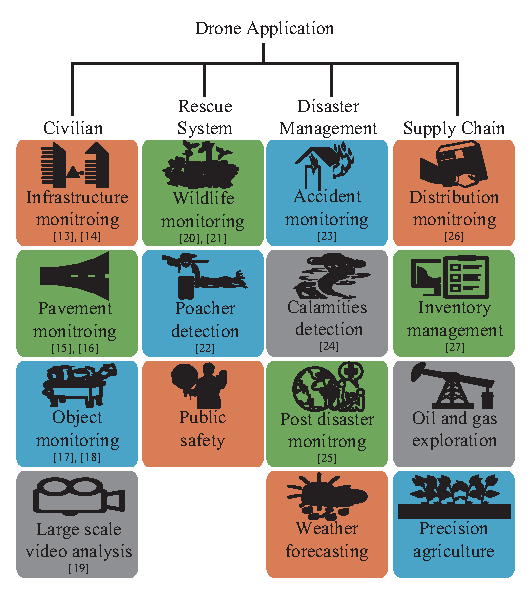
\includegraphics{figure/applicaitonfig.eps}
% \caption{Evaluation of commercial drone usage.}
% \label{applicaitonfig}
% \end{figure}
\section{Networking, Localization, and Data Management Framework for Drone}
\label{networkingsection}
%Navigation, networking, localization

For autonomous drone-based monitoring, the prerequisite is a self-operating framework.
Two crucial factors that need to be considered for autonomous operation is speed, and safety. Beside data management is another important factor.

\subsection{Autonomous Navigation}
In the known environment, a drone can avoid obstacles easily. While in an unknown environment, it is difficult to operate. In the majority case, either the system is safe but slow, or the system works fast but unsafe. In very recent research a system has been implemented that can operate independently in an unknown environment safely, with a good speed. The real world with drone's perspective can be divided into two parts; the flying zone of the drone and the outside map area. A map with a drone's perspective is shown in Fig~\ref{autonomous}. They have partitioned the flying zone area into 3 spaces~\cite{tordesillas2019real, tordesillas2019faster}. The first one is known free space (F) which is the instructed space with no construction change. The second space is known but occupied space (O) which can be represented by the change in construction or the intervene of any real-world object such as a bird. And the last one is the unknown space (U) that might be required based on the real-world situation.
\begin{figure}[h!]
\centering
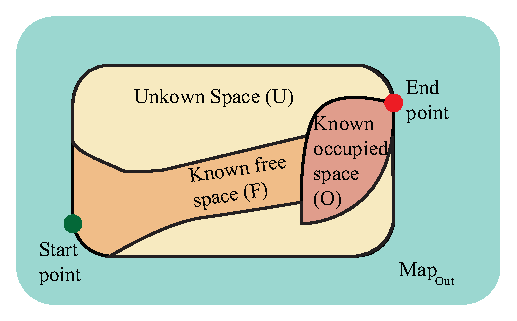
\includegraphics[width=.8\linewidth]{figure/autonomous.eps}
\caption{Flying map with drone perspective.}
\label{autonomous}
\end{figure}

In the proposed system by the authors in~\cite{liu2017planning}, Jump Point Search (JPS) is used as an universal planner to find the shortest possible route from the starting point to the ending point~\cite{harabor2011online}. Another alternative technique is A\(^*\) search but JPS not only ensures faster magnitude but also guarantees the completeness and optimality. This hierarchical input control consists of three parts i.e., a part controlled by jerk, a part controlled by velocity, and a part controlled by geometry. By using the map, the collision search for each of the three primitives shown above the whole performance can be summarized as follows. If it does not collide, the jerk operated trajectory is treated as collision-free. The velocity-controlled primitive is forced to traverse the JPS solution's paths. Eventually, a no-hit obstacle is confirmed to hit the JPS route. 
% The cost for the planned trajectory is calculated by the following equations.
% $$\text{Cost}=J_{\text{Prim}_{j}}+J_{\text{Prim}_{v}}+J_{\text{Prim}_{d}}$$

% Here, $J_{\text{Prim}_{j}}$ represents jerk-controlled primitive, $J_{\text{Prim}_{v}}$ is combination of multiple primitives regulated by velocity, and $J_{\text{Prim}_{d}}$ is the portion of JPS.

Besides, a monocular camera based drone system was proposed, where can operate autonomously in the preceding unknown indoor hallway area, where GPS is not working properly~\cite{padhy2018deep}. They have used the CNN model to reach the goal. Video captured by the camera is fed to the model, then the model takes the decision. The CNN model is designed with 4 convolutional layers and 4 pooling layers. The output of the model is left, right, and straight.

A deep learning-based network was experimented on a little shaped drone, where the drone was able to navigate autonomously in many different circumstances, e.g., a  relatively straight forest trail with 100 m length, a  zigzag forest path with 6 turns, a 1 km mountainous zigzag forest path, and an open field~\cite{smolyanskiy2017toward}. The network namely TrailNet is inspired by sResNet-18. SResNet-18 is basically a ResNet-18 with batch normalization and shifted Relu function is used instead of Relu fucntion \cite{he2016deep}. Input of the TrailNet is the image capured by the drone and outputs of the model are view orientation and lateral offset. By using these two output parameters the drone can fly indepnedently. Besides, they have also implemented safety feature for the drone, e.g., obstacle detection and avoidance.

In the racing track, a drone have to pass though several square gates. As all the gates look exactly same, and one gate is visiable through others, it is a very diffcullt task to dected the nearest gate.A ADRNet (Autonoumous Drone Racing Network) was developed for this purpose~\cite{jung2018perception}. ADRNet  is a CNN based network. Using this network and line-of-sight guidance algorithm they developed a drone system, that can comeplete a race track. 

\subsection{Safety Features}
In practical life, a drone may encounter unexpected obstacles such as a ball coming toward it, which can cause damage to the drone. Besides, covering 360$^{\circ}$ safety is not only costly but also computation expensive too. Therefore, one possible solution is using sonar sensors embedded with the drone. One of the possible solutions is utilizing the Doppler effect~\cite{garg2020enabling}. According to the formula, a drone can detect Doppler shift for a nearby moving obstacle coming towards the drone with $v_{\circ}$ speed and an $\theta$ angle with the drone then the doppler shift will be, $$\Delta f=f_{\circ} \frac{2 v_{\circ} \cos (\theta)}{v}$$ 


%if a sound source with $f_{\circ}$ coming towards an object with a $v_s$ velocity, then the frequency experienced by the object will be $$f=f_{\circ} \frac{v+v_{s}}{v-v_{t}}$$

% Here, $v$ and $v_t$ are the speed of sound and target respectively. However, with a stationary sound source and microphone system as shown in Fig~\ref{safety}, a drone can detect Doppler shift for a nearby moving obstacle coming towards the drone with $v_{\circ}$ speed. According to the theorem, the total Droppler shift will be, $$\Delta f=f_{\circ} \frac{2 v_{\circ}}{v-v_{\circ}}\approx f \frac{2 v_{\circ}}{v} \left[\text{as } v_{\circ}<<v\right]$$

\begin{figure}[h!]
\centering
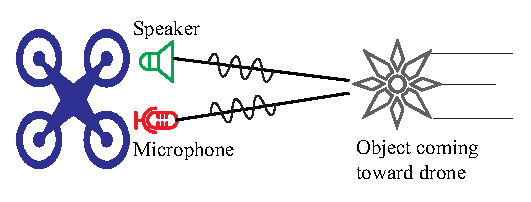
\includegraphics[width=.8\linewidth]{figure/safety.eps}
\caption{Doppler effect on drone.}
\label{safety}
\end{figure}

% Considering the velocity direction, if the moving object makes an $\theta$ angle with the drone, then only the cosine component of the object's velocity will influence the doppler shift. On that case, $$\Delta f=f_{\circ} \frac{2 v_{\circ} \cos (\theta)}{v}$$ 

A stationary sound source and microphone system as shown in Fig~\ref{safety}, a drone can detect Doppler shift for a nearby moving obstacle coming towards the drone with $v_{\circ}$ speed. However in practice, the doppler shift deviates from the ideal value because of various factors such as environmental drag. Therefore, instead of estimating the Doppler effect, the change of the effect is calculated with respect to $\Delta $ time. As $v_{\circ}$ and $\theta$ are both functions of time, the ratio will be, $$\frac{\Delta f(t+\Delta t)}{\Delta f(t)} \approx \frac{\cos \left[ \theta(t+\Delta t)\right]}{\cos \left[\theta(t)\right]}$$

This angle ratio is the changing rate of radial angle. If the value is constantly one over multiple time segments, then it means an object is coming towards the drone, that might hit it. For other non-constant values, it is safe. Therefore, utilizing this value the drone can improve its safety mechanism and dodge any harmful materials coming towards it.

Another important safety feature is safe landing. A safeUAV-nets has been proposed which make the landing safer for the drone~\cite{marcu2018safeuav}. The main task of this net is to identify the Horizontal area such as a rooftop, plain ground, in other words, a safe landing spot. For this purpose RGB camera has been used. The safeUAV-nets not only predict the safe landing ground but also estimate the depth from the UAV to the ground.

Besides a reinforcement learning-based obstacle avoidance model was proposed for the drone~\cite{singla2019memory}. The base of this model is the recurrent neural network and temporal attention. They have adopted cGAN for depth estimation. Such depth maps are feed to reinforcement with RNN (LSTM) model and the model returns the flight command. The reward function of the learning is designed by taking into account the aerial systems power consumption and the time factor in navigation operations. Though depth is predicted from unseen material world images, the output is noisy.

\subsection{Signal Processing and Data Management}
One of the major limitations in the field of machine learning is the limited space of an embedded system. So, it is important to store data more efficiently. One common technique is data compression while recording. 
A technique has been proposed that is motivated by \cite{hitomi2011video} imaging methodology to increase the frame rate of a normal off-the-shelf camera by using a silicon liquid crystal to compressively attain video-coded snapshots~\cite{kumar2018onboard}. Compression is performed out by using coded aperture imaging on a given hyperspectral datacube. For decompression, hey suggest a sparse recovery algorithm based on a deep neural network to rebuild the datacube from compressively coded snapshots. Whereas, this form of sparse data acquisition is usually decompressed using  sparse recovery algorithms such as orthogonal matching or iterative hard threshold, which is very slow process.

Another scheme to increase the working efficiency of the model is data augmentation. A method can generate sensor data of various kinds, such as camera images or Lidar point clouds~\cite{milz2018aerial}. The fundamental idea is to use a cGAN and the desired ground truth can be fed to any model as conditional input.
A two-stream CNN technique was presented that can predict the depth without using any depth sensor~\cite{kouris2018learning}. The network takes consecutive RGB image frames as input and returns the distance of any object from the drone in three directions. The CNN network is trained with a custom dataset where the actual distance from the object to the drone was collected using external HC-SR04 Ultrasonic Sensor and GP2Y0A60SZLF Analog IR Sensor mounted on the drone.
%\section{Signal Processing and Data Management Framework for Drone}
\label{signalprocessingsection}
One of the major limitations in the field of machine learning is the limited space of an embedded system. So, it is important to store data more efficiently. One common technique is data compression while recording. 
A technique has been proposed that is motivated by \cite{hitomi2011video} imaging methodology to increase the frame rate of a normal off-the-shelf camera by using a silicon liquid crystal to compressively attain video-coded snapshots~\cite{kumar2018onboard}. Compression is performed out by using coded aperture imaging on a given hyperspectral datacube. For decompression, hey suggest a sparse recovery algorithm based on a deep neural network to rebuild the datacube from compressively coded snapshots. Whereas, this form of sparse data acquisition is usually decompressed using  sparse recovery algorithms such as orthogonal matching or iterative hard threshold, which is very slow process.

Another scheme to increase the working efficiency of the model is data augmentation. A method can generate sensor data of various kinds, such as camera images or Lidar point clouds~\cite{milz2018aerial}. The fundamental idea is to use a cGAN and the desired ground truth can be fed to any model as conditional input.
A two-stream CNN technique was presented that can predict the depth without using any depth sensor~\cite{kouris2018learning}. The network takes consecutive RGB image frames as input and returns the distance of any object from the drone in three directions. The CNN network is trained with a custom dataset where the actual distance from the object to the drone was collected using external HC-SR04 Ultrasonic Sensor and GP2Y0A60SZLF Analog IR Sensor mounted on the drone.
\section{Machine learning based Drone application}
\label{applicationsection}
In the last few years, drone technology has grown and flourished on a large scale. Starting from small package delivery, drones are being used for various purposes nowadays. %Evaluation of commercially drone usage is shown in Fig~\ref{applicaitonfig}.
Though the commercial drone industry is new, it is getting a lot of attention and investments in recent years. Various research is going on regarding this purpose. Few are mentioned below.

\subsection{Inspection, Detection and Tracking}
Autonomous infrastructure inspection is one of the popular applications of UAVs. The drone provides us the advantage of frequent construction monitoring facilities with a low maintenance cost, as it can capture large scale aerial images with a very less amount of human intervention.
A transfer learning-based has developed for crack detection~\cite{kucuksubasi2018transfer}.  Their system can also navigate autonomously in a GPS denied enviornment. They have used RGB and LIDAR cameras for environment detection, and an onboard IMU sensor to detect the velocity of the drone. They have developed an open-source software for moving strategies of the drone. For crack detection, they finetuned different architecture of the CNN model. Among them, InceptionV3 has performed better than others.
In another system the UAV operates autonomously using an ultrasonic beacon system instead of GPS~\cite{kang2018autonomous}. In this research, they developed a ground system that detects the position data from a beacon data using an extended Kalman filter 3 (EKF3) algorithm \cite{willner1976kalman}. This position data is fed to the PID system, which controls the UAV. For crack detection, this system has used CNN with a sliding window technique \cite{cha2017deep}.

Another domain of inspection is road or pavement monitoring. In the CNN and RNN based pavement monitoring system~\cite{wu2018coupling}, they have detected the crack of the pavement using different CNN models, such as Faster Regional-CNN \cite{ren2015faster}, YOLO \cite{redmon2016you}, and Single Shot Multi-Box Detector (SSD) \cite{liu2016ssd}. The output of the model is the rating of the pavement condition, which is fed to an RNN to model to identify the location information. They have used RGB and IR thermal camera.
Transformed image can also be used instead of raw image for road inspection~\cite{fan2019real}. In that research they have converted the perspective view into reference view. Their whole work is divided into three part: perspective transformation (converting image same as reference), dense road stereo (cost computation with reference), and finally disparity transformation. Using this algorithm results in computational complexity reduction of the algorithm and disparity accuracy improvement. 

For most of the drone-based detection case, most of the researcher works on static objects. Very few research explored the model of motion. For this purpose, a benchmark dataset was constructed consisting of 70 videos~\cite{li2017visual}. They have introduced a new camera motion $\mathbf{H}_{t}$ term is in the motion model $\mathbf{z}_{t}=\mathbf{H}_{t} \mathbf{z}_{t-1}+\Delta \mathbf{z}_{t}$. As a baseline of the tracking system, they used the following methods: three types of correlation filter approaches (KCF~\cite{henriques2014high}, DSST~\cite{danelljan2014accurate}, SRDCF~\cite{danelljan2015learning}), color-based discriminatory tracker (DAT~\cite{possegger2015defense}); approach based on a competitive particle filter (HOGLR~\cite{wang2015understanding}); ensemble technique (MEEM~\cite{zhang2014meem}); and two approaches, based on deep learning (SODLT~\cite{wang2015transferring}, MDNet~\cite{nam2016learning}). Several other methods were proposed to detect and track a UAV using another UAV. For example, YOLOv3 and YOLOv3-Tiny models had been utilized for detection purpose~\cite{saribas2019hybrid}. Their main contribution is introducing a kernelized  correlation filter which improves the detection result. 

The analysis of videos captured by drones for the extraction of useful information is complicated because of the presence of small items, changes in viewpoints of these items, changes in lighting, large-scale video resolution, occlusion, and truncation. To overcome these challenges, a processing pipeline  was proposed integrating DeForm convolution layers in the backbone~\cite{zhang2019dense}.

\subsection{Disaster Management, Rescue System, and Supply Chain}
A drone can be an efficient tool in case of a rescue mission. Rescue programs are often involved in remote operations, treating the sick, or searching for missing people. Time is an essential factor in making search and rescue missions a positive outcome.  The rescue and search operation of wildlife is more challenging~\cite{mayer2019drones}. According to the research~\cite{brennan2019drones}, in case of these operations, the model should have few qualities, E.g., guidance and navigation; collaborative search and inspection; physically handling materials.
SPOT (Systematic Poacher Detector) which increases the capacity of drones to automatically identify poachers and animals in near real-time~\cite{bondi2018spot}.  SPOT uses state-of-the-art AI strategies, such as Faster RCNN as the base model, where input is the infrared image.

A framework  was outlined for creating explanations of autonomous system behavior and reasoning~\cite{garcia2018explainable}. They focused on the NLP for explaining incidence. They have named their model as 'speak-aloud,' which can fly to a remote area and alert if any accident occurs. In short, it is a chatbot that will not only describe the incident but also can reply to the different questions of users on that incident. For a vehicle spiraling incident, if a user asks why it is doing like this, the system will respond with the reason behind that (E.g., GPS fixing or transmitting to safe plane depth).

A autonomous drone can monitor a area and detect various calamities like flood, fire, collapsed building~\cite{kyrkou2019deep}. They have introduced a Aerial Image Database for Emergency Response application which is named as AIDER. Based on the analysis of the database, they have built a light weight CNN architecture on a embedded device.
Another system namely ``DronAID'' is capable of identifying people in desperate circumstances~\cite{tariq2018dronaid}. They have detected humans using a PIR sensor of the drone. According to the \cite{jin2011target}, a human body radiates IR at a certain wavelength. Besides detecting humans, this DronAID can also telecast a live stream and provide the location of the trapped person to the rescue team. 

The supply chain is a sequential process that is associated with the production and distribution of commercial goods. Nowadays, UAVs have a lot of applications in autonomous supply chain management. An image processing system has been introduced that can classify, quantify the number of citrus fruits from every single tree of a garden~\cite{apolo2020deep}. It can also predict the shape of each fruit using deep learning. They have used a Faster R-CNN Deep Learning model to detect orange. They have also used an LSTM model to predict the possible number of orange in advance. They conducted this experiment on 20 trees for three consecutive years.

A company needs to keep track of its stock to succeed in the market. For this purpose, a drone can be used to perform a periodic inventory check and determine whether to purchase more supplies. According to the concept of Industry 4.0, a drone-based system has been developed to automate inventory stuff and keep the record of products assigned by the RFID tags~\cite{fernandez2019towards}. The framework uses a blockchain and a distributed ledger to store and verify all product data obtained by the drone. 
\section{Drone Related Dataset}
\label{datasetsection}
Drone with RGB cameras has a broad range of applications, including aerial photography, agriculture, civil construction inspection, and monitoring. Additionally, an autonomous understanding system of the visual data collected from these platforms is becoming highly demanding, thus increasingly bringing computer vision to drones. Some datasets regarding drone are provided below and summerized in Table~\ref{datatable}.

\begin{table*}[h] 
\centering
\caption{Dataset related to drone}
\begin{tabular}{|l|l|l|l|l|}
\hline
Dataset                                                                                                                    & Drone                                                                                          & Resolution (Px)                                                                             & Instances                                                                                                               & Applications                                                                                                                                                      \\ \hline
\begin{tabular}[c]{@{}l@{}}Visdrone\\\cite{zhu2018vision, zhu2020vision} \end{tabular}                                                                                                                   & \begin{tabular}[c]{@{}l@{}}DJI Mavic,\\ DJI Phantom\\ (3, 3A, 3SE, 3P, 4, 4A, 4P)\end{tabular} & \begin{tabular}[c]{@{}l@{}}video 3840 $\times$ 2160\\ image 2000 $\times$ 1500\end{tabular} & \begin{tabular}[c]{@{}l@{}}Video 263\\ Image 179,264\end{tabular}                                                       & \begin{tabular}[c]{@{}l@{}}Object detection from image and\\ video, object tracking both single and\\ multi-object.\end{tabular}                                  \\ \hline

\begin{tabular}[c]{@{}l@{}}Car Parking Lot\\ Dataset (CARPK)\\ \cite{hsieh2017drone}\end{tabular}                                                  & Phantom 3 Professional                                                                         & 1280 $\times$  720                                                                          &                                                                                                                         & Detection and objects count                                                                                                                                       \\ \hline

\begin{tabular}[c]{@{}l@{}}The Unmanned Aerial\\ Vehicle Benchmark:\\ Object Detection and\\ Tracking (UAVDT)\\ \cite{du2018unmanned}\end{tabular} & DJI Inspire 2                                                                                  & 1080 $\times$ 540                                                                           & \begin{tabular}[c]{@{}l@{}}10 hr raw videos\\ 80,000 frames\end{tabular}                                                & \begin{tabular}[c]{@{}l@{}}Object detection, single-object tracking,\\ and multiple object tracking. Here\\ object  means vehicles (Car, truck, bus)\end{tabular} \\ \hline

\begin{tabular}[c]{@{}l@{}}Aerial Image Dataset for\\ Emergency Response\\ dataset (AIDAR)\\ \cite{kyrkou2019deep, kyrkou2020emergencynet}\end{tabular}                    & DJI Matric 100                                                                                 & 128 $\times$ 128                                                                            & \begin{tabular}[c]{@{}l@{}}370 images flood\\ 320 images rubble\\ 335 images accident\\ 1200 images normal\end{tabular} & \begin{tabular}[c]{@{}l@{}}Disaster detection, such as fire, flood,\\ collapsed building, traffic accidents\end{tabular}                                          \\ \hline

\begin{tabular}[c]{@{}l@{}}SafeUAV \\ \cite{marcu2018safeuav}     \end{tabular}                                                                                                              &                                                                                                & \begin{tabular}[c]{@{}l@{}}RGB 640 $\times$ 480\\ also depth image\end{tabular}             & \begin{tabular}[c]{@{}l@{}}Urban 6.8 km$^2$\\ 8101 samples\\ Suburban 2.8 km$^2$\\ 3770 samples\end{tabular}            & \begin{tabular}[c]{@{}l@{}}Whether a place is safe for drone \\ landing or not\end{tabular}                                                                       \\ \hline


\begin{tabular}[c]{@{}l@{}}  HighD \\ \cite{krajewski2018highd} \end{tabular}      &  DJI Phantom 4 Pro Plus                                                                                             & \begin{tabular}[c]{@{}l@{}}Video 4096 $\times$ 2160\\ at 25 fps\end{tabular}             & \begin{tabular}[c]{@{}l@{}}110,500 vehicles\\ 45,000 km area\end{tabular}            & \begin{tabular}[c]{@{}l@{}}Analyze the traffic pattern in \\ German highway \end{tabular}                                                                       \\ \hline


\begin{tabular}[c]{@{}l@{}}High Resolution UAV \\ Dataset (HRUD) \\ \cite{rahnemoonfar2020comprehensive, rahnemoonfar2020floodnet}      \end{tabular}      &                                                                                              & 3000 $\times$ 4000            & \begin{tabular}[c]{@{}l@{}}2000 images\end{tabular}            & \begin{tabular}[c]{@{}l@{}}Recognition and better understanding\\ of post disaster situations \end{tabular}                                                                       \\ \hline



\begin{tabular}[c]{@{}l@{}}Stanford Drone Dataset    \\ \cite{robicquet2016learning}    \end{tabular}                                                                                             & 3DR Solo with 4k camera                                                                        & 1400 $\times$ 1904                                                                          & \begin{tabular}[c]{@{}l@{}}Approx 920k frames\\ consisting of 19k\\ target\end{tabular}                                 & \begin{tabular}[c]{@{}l@{}}Target trajectory prediction including\\ social etiquettes and common sense\\ actions; multitarget tracking\end{tabular}               \\ \hline

\begin{tabular}[c]{@{}l@{}}Autonomous Drone\\ Racing Dataset \\ \cite{jung2018perception}\end{tabular} & \begin{tabular}[c]{@{}l@{}}Custom made with\\ NVIDIA TX1\end{tabular} & Video Speed 30 fps & \begin{tabular}[c]{@{}l@{}}Training 1544 frames\\ testing 7380 frames\end{tabular} & \begin{tabular}[c]{@{}l@{}}Autonomus drone racing track\\ completion\end{tabular} \\ \hline

\begin{tabular}[c]{@{}l@{}}Crashes Itself!     \\ \cite{gandhi2017learning}    \end{tabular}                                                  & Parrot AR.Drone 2.0                                                   & 1280 $\times$ 720  & 11,500 crashes                                                                     & \begin{tabular}[c]{@{}l@{}}Drone hit obstacles. Data was \\ annotated as positive or negative\\ while collecting the crashing data.\end{tabular} \\ \hline

\end{tabular}
\label{datatable}
\end{table*}

\subsection{Visdrone}
Visdrone is one of the large benchmark datasets that is prepared by a research team of Machine Learning and Data Mining Lab, Tianjin University, China. This dataset is related to computer vision and captured by a drone. Data were collected from 14 different sites in China. The dataset covers numerous weather and lighting conditions, reflecting various situations in our daily life. There are 10 labeled object categories (pedestrian, vehicles, bicycles, etc.), and density conditions are sparse and crowded scenes. There are two object detection tasks (detection from image and detection from video), and two object tracking tasks (single-object tracking and multi-object tracking). Based on this dataset, two competitions were organized, namely VisDrone 2018 and VisDrone 2019 in collaboration with ECCV 2018 and ICCV 2019, respectively. VisDrone 2020 will be held with a new difficulty, crowd counting.


\subsection{Car parking lot dataset (CARPK)}
Similar to the name of the dataset, the car parking lot dataset or CARPK concentrates on the number of cars parked in a parking lot. Therefore, vehicle detection and counting is the only challenge in this dataset. The dataset includes almost 90,000 annotated bounding boxes of cars. The dataset contains 4 different parking lot scenarios with drone view at an altitude of approximately 40 metres.

\subsection{The Unmanned Aerial Vehicle Benchmark: Object Detection and Tracking (UAVDT)}
The Unmanned Aerial Vehicle Benchmark: Object Detection and Tracking (UAVDT) consist of 10 hours of video data. Those frames are fully annotated with bounding boxes. Labels of those bounding boxes are vehicles such as car, truck, and bus. The primary task of the dataset is object detection, which can be either single object tracking or multiple object tracking.  The videos were shot in multiple lighting conditions (daylight, night, and fog). Different lighting conditions introduce different aspects. Daytime light introduces shadow interaction with the object. Whereas, night scene, with dim street lamplight, offers barely any information about texture. Meanwhile, frames captured at fog lose sharp details so that object contours disappear in the background.

\subsection{Aerial Image Dataset for Emergency Response dataset (AIDAR)}

This dataset consists of photographs for four different disaster events, such as flood, fire/smoke, traffic accidents, collapsed building/rubble disaster. Additionally, it also contains common cases that do not indicate the existence of a disaster. Besides, collecting images using their UAV platform (DJI Matric 100), the aerial photos of these types of disasters were obtained from various sources, such as twitter, bing images, websites of news agencies, google images, etc.

\subsection{SafeUAV}

The task of this dataset is to identify the condition of the landing ground, e.g., horizontal, vertical, or sloped. In short, whether a drone can land on that ground or not. In the SafeUAV dataset, data have been collected from two types of places. From Urban A and Urban B, this dataset covered 3.5 km$^2$ and 3.3 km$^2$, consisting of 4545 samples and 3592 samples from those areas. Similarly, from Suburban A and Suburban B, this dataset covered 1.7 km$^2$ and 1.1 km$^2$, consisting of 2458 samples and 1312 samples. This dataset consists of an RGB image, a precise depth measure for individual pixels. For ground truths of the label, the 3D model of the base have imperfections, such as containing several reconstruction inconsistencies. The actual output of the dataset, however, is still not pragmatic.

\subsection{HighD}
This dataset was created on German highways by filming the naturalistic trajectories of vehicles using a drone. The purpose of using a drone is to solve the problem of occlusions and get an aerial perspective view that is tough to get by grounded data. This dataset consists of more than 110 500 transportations with the truck and car class. The video was capture in six different places and at 4K resolution with 25 fps. Four types of maneuvers (free driving, vehicle following, critical maneuver, lane change) were also annotated in this dataset.

\subsection{High Resolution UAV Dataset (HRUD)}
This dataset was captured for information processing in the post-Hurricane Michael disaster scenario. There are around 2000 aerial photographs with semantic segmentation data annotation. Data were collected after Hurricane Michael. Three types of damage are labeled in this dataset (No Damage, Medium Damage, Major Damage).


\subsection{Stanford Drone Dataset}

The dataset consists of around 920 thousand frames, which includes approximately 19 thousand targets involving 11,200 pedestrians, 6,400 bicycle riders, 1,300 vehicles, 300 skaters, 200 golf carts, and 100 buses. This dataset aims to predict social etiquettes while a large number of people are on the street, which means the interactions between two targets and between target and space. Such as trajected of a pedestrian and a cyclist should not crossover. Based on this assumption, they tried to predict the trajectory of humans in different areas of the campus. There are 185 thousand annotated interactions between two targets and 40 thousand annotated interactions between a target and space. The dataset was collected from 8 different places of Standford University.


\subsection{Autonomous Drone Racing Dataset}

This dataset was created using a fisheye camera mounted on a drone. The Field-of-View of the camera was 170$^{\circ}$. The dataset is consists of gates used in a drone racing track. Data was captured by the frontal camera the drone and video quality was VGA. The data capture rate was 30 Hz. The primary motivation of the dataset is to develop an algorithm for an autonomous racing drone.


\subsection{Crashes Itself!}

In the field of autonomous drone navigation, very research work created a dataset, where a drone actually hit an obstacle. Most of the crash datasets are synthetically prepared. In this dataset, the researchers have crashed their drones for 11.5 thousand times. For video capturing purposes, they have used a Parrot Ar-Drone 2.0 with slight modification. Besides, a software was implanted on the drone so that it could autonomously crash into obstacles and recover from the consequences. Data is annotated as the positive class and negative class.
\section{Drone Related Hardware}
\label{toolkitsection}
In real life, there are multiple constraints and restrictions. To successfully implement ideas, all of these limitations should be taken into consideration. Specifically, for using a deep learning-based approach on a drone, sensing systems, and communications design constraints should be investigated intensively~\cite{fraga2019review}. The hardware factors of a drone are shown in Fig~\ref{hardware}. These factors are discussed below.
\begin{figure}[h!]
\centering
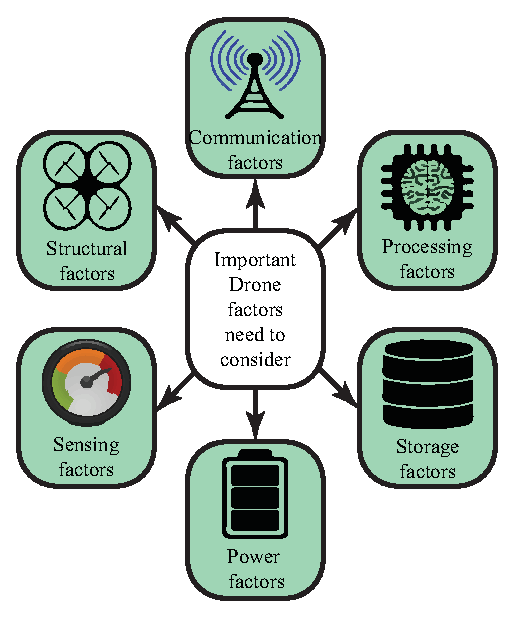
\includegraphics[width=.7\linewidth]{figure/hardware.eps}
\caption{Factors need to be considered before using drone.}
\label{hardware}
\end{figure}
\subsection{Communication Factors}
The most important part of the drone is the communication system. RFID and WIFI are the most commonly used communication protocols for drones. Another popular alternative to these protocols is Bluetooth, as Bluetooth consumes less power then WIFI. But the advantage of WIFI over Bluetooth is the high data transmission and receiving rate. But both of these protocols can not be used for long-range communication. For that purpose, cellular networks can be used. Based on the communication range, frequency bandwidth, data transmission rate, and power consumption criteria, we need to select the communication protocol. There are many communication protocols, such as Zigbee, Z-wave, NFC (narrow field communication), etc. In Table~\ref{communicationprotocol}, we have provided a few communication protocols used for drone communication.
\begin{table}[h]
\scriptsize
\centering
\caption{Wireless communication protocols for drone}
\begin{tabular}{@{}|l|l|l|l|l|@{}}
\toprule
          & Band                                                                             & Range                                                   & Data rate                                                      & \begin{tabular}[c]{@{}l@{}}Power\\ consumption\end{tabular} \\ \midrule
Wifi      & \begin{tabular}[c]{@{}l@{}}900MHz, 2.4GHz, 3.65\\ GHz, 5GHz, 5.9GHz\end{tabular} & 100m                                                    & \begin{tabular}[c]{@{}l@{}}2Mbps to\\ 54Mbps\end{tabular}      & high                                                        \\ \midrule
Bluetooth & 2.4GHz                                                                           & 250m                                                    & upto 2Mbps                                                     & low                                                         \\ \midrule
Zigbee    & 2.4GHz                                                                           & \begin{tabular}[c]{@{}l@{}}10m to\\ 100m\end{tabular}   & 100kbps                                                        & very low                                                    \\ \midrule
Z-wave    & 900MHz                                                                           & 30m                                                     & 100kbps                                                        &                                                             \\ \midrule
6LoWPAN   & \begin{tabular}[c]{@{}l@{}}2.4GHz or\\ 900MHz\end{tabular}                       & \begin{tabular}[c]{@{}l@{}}10m to\\ 100m\end{tabular}   & 250kbps                                                        & low                                                         \\ \midrule
RF        & \begin{tabular}[c]{@{}l@{}}starts from KHz and\\ ranges till GHz\end{tabular}    & \begin{tabular}[c]{@{}l@{}}10cm to\\ 200m\end{tabular}  & \begin{tabular}[c]{@{}l@{}}depends on\\ frequency\end{tabular} &                                                             \\ \midrule
Cellular  & 900MHz to 2100MHz                                                                & \begin{tabular}[c]{@{}l@{}}35km to\\ 200km\end{tabular} & \begin{tabular}[c]{@{}l@{}}35Kbps to\\ 10Mbps\end{tabular}     & Very high                                                   \\ \midrule
NB-IOT    & 200KHz                                                                           & 10Km                                                    & 250kbps                                                        & low                                                         \\ \midrule
5G        & 6GHz                                                                             & 500m                                                    & 1Gbps                                                          & Very high                                                   \\ \midrule
NFC       & 13.56MHz                                                                         & 10cm                                                    & \begin{tabular}[c]{@{}l@{}}100kbps to\\ 420kbps\end{tabular}   & low                                                         \\ \midrule
LoRaWAN   & 2.4GHz                                                                           & \begin{tabular}[c]{@{}l@{}}2km to\\ 5km\end{tabular}    & \begin{tabular}[c]{@{}l@{}}0.3kbps to\\ 50kbps\end{tabular}    & Very low                                                    \\ \bottomrule
\end{tabular}
\label{communicationprotocol}
\end{table}




% \begin{table}[h]
% \centering
% \caption{Wireless communication protocols for drone}
% \begin{tabular}{|l|l|l|l|l|}
% \hline
%             & Band                                                                                  & Range                                                           & Data rate                                                      & \begin{tabular}[c]{@{}l@{}}Power\\ consu-\\ mption\end{tabular} \\ \hline
% WIFI        & \begin{tabular}[c]{@{}l@{}}900MHz, 2.4GHz,\\3.65GHz, 5GHz,\\ 5.9GHz\end{tabular}                            & 100m                                                        & \begin{tabular}[c]{@{}l@{}}2Mbps\\ to\\ 54Mbps\end{tabular}    & high                                                            \\ \hline
% Bluetooth   & 2.4GHz                                                                                & 250m                                                       & \begin{tabular}[c]{@{}l@{}}upto\\ 2Mbps\end{tabular}           & low                                                             \\ \hline
% Zigbee      & 2.4GHz                                                                                & \begin{tabular}[c]{@{}l@{}}10m\\ to\\ 100m\end{tabular}   & 100kbps                                                        & \begin{tabular}[c]{@{}l@{}}very\\ low\end{tabular}              \\ \hline
% Z-wave      & 900MHz                                                                                & 30m                                                                                                          & 100kbps                                                        &                                                                 \\ \hline
% 6LoWPAN     & \begin{tabular}[c]{@{}l@{}}2.4GHz\\ or\\ 900MHz\end{tabular}                          &        \begin{tabular}[c]{@{}l@{}}10m\\ to\\ 100m\end{tabular}                                                   &     250kbps                                                           & low                                                             \\ \hline
% RF          & \begin{tabular}[c]{@{}l@{}}starts\\ from\\ KHz\\ and\\ ranges\\ till GHz\end{tabular} & \begin{tabular}[c]{@{}l@{}}10cm\\ to\\ 200m\end{tabular}                                                         & \begin{tabular}[c]{@{}l@{}}depends\\ on\\ frequency\end{tabular}       &                                                                 \\ \hline
% Cellular    & \begin{tabular}[c]{@{}l@{}}900MHz\\ to\\ 2100MHz\end{tabular}                         & \begin{tabular}[c]{@{}l@{}}35km\\ to\\ 200km\end{tabular} &                                                          \begin{tabular}[c]{@{}l@{}}35Kbps\\ to\\ 10Mbps\end{tabular}   &       \begin{tabular}[c]{@{}l@{}}Very\\ high\\\end{tabular}        \\ \hline
% NB-IOT      &         200KHz                                                                              & 10Km                                                                                                               & 250kbps                                                        & low                                                             \\ \hline
% 5G          & 6GHz                                                                                  &        500m                                                                                                            & 1Gbps                                                          &    \begin{tabular}[c]{@{}l@{}}Very\\ high\\\end{tabular}                                                              \\ \hline
% NFC         & 13.56MHz                                                                              & 10cm                                                                                                              & \begin{tabular}[c]{@{}l@{}}100kbps\\ to\\ 420kbps\end{tabular} &                     low                                            \\ \hline
% LoRaWAN     & 2.4GHz                                                                                & \begin{tabular}[c]{@{}l@{}}2km\\ to\\ 5km\end{tabular}                                                           & \begin{tabular}[c]{@{}l@{}}0.3kbps\\ to\\ 50kbps\end{tabular}  &   \begin{tabular}[c]{@{}l@{}}Very\\ low\\\end{tabular}                                                              \\ \hline
% %LTE-M       &                                                                                       &                                                           &                                                         & \begin{tabular}[c]{@{}l@{}}100kbps\\ to\\ 375kbps\end{tabular} &                                                                 \\ \hline
% \end{tabular}
% \label{communicationprotocol}
% \end{table}

\subsection{Sensor Factors}
Sensors play a crucial role in drone navigation and data capture. Those sensors help the drone to collect data from the surroundings. Using this knowledge, a drone can maintain its positions, decide how fast it is moving, and avoid barriers. Commonly used drone sensors are mentioned below.

\textbf{RGB camera:} 
The most commonly attached sensor in a drone is an RGB camera. An RGB camera is required to provide drone pilots with feedback. Besides, a range of creative and realistic applications are found with drone cameras these days. Among them, autonomous navigation, wildlife surveillance, weather forecasting, archaeological surveys, aerial photography are notable. Depending on the price, drone cameras can vary in quality and size.

\textbf{Thermal camera:}
A thermal camera can transform the drone into a versatile device that can be used in many sectors, such as quarrying, energy monitoring, health inspection, firefighting, etc. The thermal camera uses vision imaging technique that can sense and transform heat coming from virtually all objects and materials into photographs. 

\textbf{Gyroscope:}
Gyroscope is inexpensive and easy enough to fit into even inexpensive mini-drones. The gyroscopes work on the principle of angular momentum conservation. This device is used to measure or maintain orientation.

\textbf{Accelerometers:}
A drone's accelerometer operates in tandem with its gyroscope to determine changes in the drone's position and motion. The working principle of an accelerometer is based on the piezoelectric effect. A gyroscope can read rotational movements, whereas an accelerometer is better able to read linear motions along any axis. 

\textbf{Tilt Sensor:}
The tilt sensor is a hybrid sensor that consists of a gyroscope and an accelerometer. The tilt sensor can provide feedback into the flight-control device to maintain level flight.

\textbf{Barometer:}
Barometers are atmospheric pressure measuring instruments. By using the atmospheric pressure, a drone can determine it's altitude from the ground. 

\textbf{GPS:}
Global Positioning System is an essential part of commercial drones. It plays an important role in the field of autonomous navigation. The GPS sensor communicates with the GPS satellite and detects the position based on the satellite. Then the 3D position of the drone within a given geospatial reference network is calculated by triangulating the position of the drone with respect to the various GPS satellites.

\textbf{Magnetometer:}
A magnetometer, as its name suggests, measures the direction and force of a magnetic field. Using a magnetometer, a drone can determine the strength of the magnetic and electric field and change its route consequently.

\textbf{IMU:}
Inertial Measurement Units or also known as IMU is a combined package, that consists of accelerometers, magnetometers, and gyroscopes.

\textbf{Sonar Sensor:}
The Sonar sensor uses sound waves to detect the distance between an object and the drone. By using multiple sonar sensors, the drone can avoid obstacles towards its path.

\subsection{Other Factors}
Beside embedded sensors and communication systems, we need to consider a few other factors before buying a drone. Weight, size, and maximum payload of a drone is the most important parameters because flight time mostly depends on these specifications. A professional parcel delivering drone on average can lift weighing around 40 lbs. On the other hand, the average flight time of the majority of commercial drones is 20-30 minutes. Though flight time can be increased by using a powerful battery, it must be noted that the higher the battery strength, the heavier it becomes. The bottlenecks of battery technology are Li-ion, LiPolymer, etc. However, research is still going on for a long-life battery with reduced weight. The other two important specifications are the controlling system and the storage system. Commonly used microprocessors are based on ARM architecture. Considering all the criteria mentioned above, a list of drones used for the educational research purpose is provided in Table~\ref{dronetable}.
\begin{table}[h]
\scriptsize
\centering
\caption{List of common drones used for research}
\begin{tabular}{@{}|l|l|l|l|l|l|@{}}
\toprule
Drone Name                                                           & \begin{tabular}[c]{@{}l@{}}Flight\\ Time\end{tabular} & Range & Camera                                                     & Other sensors                                                                        & Price (\$) \\ \midrule
DJI Mavic Pro                                                        & 27 min                                                & 7 km  & 12 MP                                                      &                                                                                      & 899        \\ \midrule
DJI Spark                                                            & 16 min                                                & 2 km  & 12 MP                                                      &                                                                                      & 455        \\ \midrule
\begin{tabular}[c]{@{}l@{}}DJI Phantom 4\\ Pro\end{tabular}          & 30 min                                                & 7 km  & 20 MP                                                      & IR sensor                                                                            & 1729       \\ \midrule
\begin{tabular}[c]{@{}l@{}}DJI Phantom 4\\ Advanced\end{tabular}     & 30 min                                                & 7 km  & 20 MP                                                      &                                                                                      & 900        \\ \midrule
DJI Inspire 2                                                        & 27 min                                                & 7 km  & \begin{tabular}[c]{@{}l@{}}No built-\\ in cam\end{tabular} & IR sensor                                                                            & 3499       \\ \midrule
\begin{tabular}[c]{@{}l@{}}DJI Matric\\ 100\end{tabular}             & 40 min                                                & 5 km  & \begin{tabular}[c]{@{}l@{}}No built-\\ in cam\end{tabular} & \begin{tabular}[c]{@{}l@{}}Pressure, GPS,\\ Magnetometer,\\ Ultra sonic\end{tabular} & 3299       \\ \midrule
\begin{tabular}[c]{@{}l@{}}YUNEEC\\ TYPHOON\end{tabular}             & 22 min                                                & 1 km  & 12 MP                                                      & Sonar sensor                                                                         & 1199       \\ \midrule
\begin{tabular}[c]{@{}l@{}}Parrot ANAFI\\ Thermal Drone\end{tabular} & 26 min                                                & 4 km  & 21 MP                                                      & \begin{tabular}[c]{@{}l@{}}GPS, Barometer,\\ Magnetometer,\\IMU\end{tabular}          & 1900       \\ \midrule
\begin{tabular}[c]{@{}l@{}}Parrot AR\\ Drone 2.0\end{tabular}        & 12 min                                                & 50 m  & HD                                                         &                                                                                      & 299        \\ \midrule
\begin{tabular}[c]{@{}l@{}}Parrot Bebop\\ 2.0\end{tabular}           & 25 min                                                & 2 km  & 14 MP                                                      & \begin{tabular}[c]{@{}l@{}}Pressure, GPS,\\ Magnetometer,\\ Ultra sonic\end{tabular} & 499        \\ \bottomrule
\end{tabular}
\label{dronetable}
\end{table}

% \begin{table*}[h]
% \scriptsize
% \centering
% \caption{List of common drones used for research}
% \begin{tabular}{|l|l|l|l|l|l|}
% \hline
% Drone Name                 & Flight Time & Range & Camera                                                    & Other sensors                                                                       & Price (\$) \\ \hline
% DJI Mavic Pro              & 27 min      & 7 km  & 12 MP                                                     &                                                                                     & 899        \\ \hline
% DJI Spark                  & 16 min      & 2 km  & 12 MP                                                     &                                                                                     & 455        \\ \hline
% DJI Phantom 4 Pro          & 30 min      & 7 km  & 20 MP                                                     & IR sensor                                                                           & 1729       \\ \hline
% DJI Phantom 4 Advanced     & 30 min      & 7 km  & 20 MP                                                     &                                                                                     & 900        \\ \hline
% DJI Inspire 2              & 27 min      & 7 km  & \begin{tabular}[c]{@{}l@{}}No built-in  cam\end{tabular} & IR sensor                                                                           & 3499       \\ \hline
% DJI Matric 100             & 40 min      & 5 km  & \begin{tabular}[c]{@{}l@{}}No built-in  cam\end{tabular} & \begin{tabular}[c]{@{}l@{}}Pressure, GPS, Magnetometer, Ultra sonic\end{tabular} & 3299       \\ \hline
% YUNEEC TYPHOON H           & 22 min      & 1 km  & 12 MP                                                     & Sonar sensor                                                                        & 1199       \\ \hline
% Parrot ANAFI Thermal Drone & 26 min      & 4 km  & 21 MP                                                     & \begin{tabular}[c]{@{}l@{}}GPS, Barometer, Magnetometer, IMU\end{tabular}         & 1900       \\ \hline
% Parrot AR Drone 2.0        & 12 min      & 50 m  & HD                                                        &                                                                                     & 299        \\ \hline
% Parrot Bebop 2.0           & 25 min      & 2 km  & 14 MP                                                     & \begin{tabular}[c]{@{}l@{}}Pressure, GPS, Magnetometer, Ultra sonic\end{tabular} & 499        \\ \hline
% \end{tabular}
% \label{dronetable}
% \end{table*}

%maybe table na top producing company https://www.businessinsider.com/drone-manufacturers-companies-invest-stocks
\section{COVID-19 AND DRONE}
\label{covid19section}
\textcolor{red}{
The novel coronavirus, known as COVID-19 has emerged as a global pandemic in 2020 and ravaged the social and economic life of the people across the globe. The ubiquitous nature of drones has proven aptly helpful in a number of use cases, from performing COVID-19 related risk assessment, monitoring to providing real-time support to citizens and authorities in a number of countries. Despite the increase in such specialized use cases, the drone industry has suffered from continued financial losses due to lower consumer space demand and reduced manufacturing capacity as a result of factory shutdowns. In this section, we briefly discuss the details of these circumstances.}
% Like other organizations, the drone industry has also suffered financial losses. 
% On the other hand, these drones helped us a lot to tackle this situation in several ways. 
% All of these will be discussed below. 
% A metaphorical picture is portrayed in Fig~\ref{dronevscovid}.
% \begin{figure}[h!]
% \centering
% 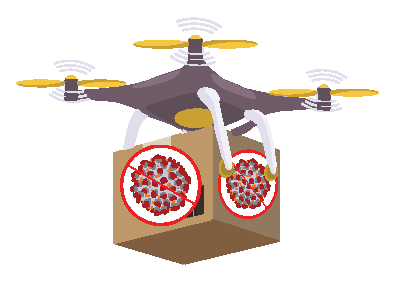
\includegraphics[width=.5\linewidth]{figure/dronevscovid.eps}
% \caption{A metaphorical picture of drone vs COVID-19.}
% \label{dronevscovid}
% \end{figure}

\subsection{Usage of Drone in COVID-19 Situation}
% The most prospective use of a drone can be possible during a pandemic situation~\cite{dronecnn}
\textcolor{red}{
The autonomous operation capabilities of drones, paired with visual and audio sensing modalities provide them with unparalleled flexibility in contactless monitoring and delivery operations. Indeed, during COVID-19 crisis, 
}
% During COVID-19, contactless delivery and autonomous vehicles are badly needed to help keep people out of risk. A drone has not only autonomous operation capabilities but also vision and hearing senses, which can monitor surroundings.
% Therefore, 
\textcolor{red}{
several countries utilized drones to carry supplies and warn their citizens. For example, during the initial stage of the pandemic, China used drones to encourage citizens to wear protective gears and masks~\cite{dronefortune}.
In Indonesia, United Arab Emirates and Spain, drones were commissioned to deploy disinfectants in areas deemed too dangerous for humans~\cite{dronefortune}.
In Saudi Arabia and Italy, authorities have been using the thermal drone to pre-screen abnormal body temperatures. Similarly, Chilean authorities have utilized drones to distribute drugs to people in remote rural areas. In the united states too, there has been an increasing trend in utilizing drones to combat the pandemic~\cite{dronefortune}. In Grand Forks, North Dakota, local Walmarts have been offering new home delivery options of food and medical supplies by drones. These examples have demonstrated that drones can be an effective aide in management of a worldwide large scale pandemic.
}
% Although drones can not measure the temperature of the body precisely, they can distinguish people with abnormal body temperatures corresponding to the surroundings. 
% In Chile, authorities have been using drones to distribute drugs to people in remote rural areas. 
% Like other nations, drones are also being used in the United States during the pandemic~\cite{dronefortune}. 
% In Grand Forks, North Dakota, local Walmarts are offering new home delivery options of food and medical supplies by drones.
% zaher: we cannot say without citations
% Some companies are interested in utilizing drones to fight the virus, e.g., spraying disinfectants in large, or searching infected people in the crowds using the thermal vision of the drone.

\subsection{Effects of COVID-19 on Drone Industry}
\textcolor{red}{
Although the usage of drones in COVID-19 management has seen a good rise, 2020 has actually proven to be a challenging years for the drone industry.
}
%\todo[inline]{change the caption: predicted value of drone industry (in billions of dollars)}
% A very challenging decade for drone industry has started in the year of 2020. 
A chart of the predicted value of drone industry in 2021 is shown in Fig~\ref{dronemarket}.
\begin{figure}[h!]
\centering
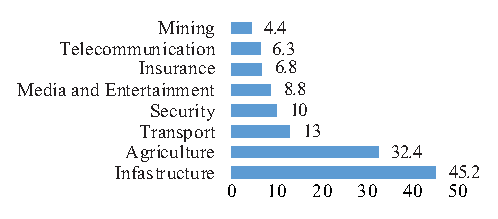
\includegraphics[width=.8\linewidth]{figure/dronemarket.eps}
\caption{Predicted value of drone industry (in billions of dollars).}
\label{dronemarket}
\end{figure}
According to the Business Insider~\cite{dronebusinessinsider}, the expected drone sale in 2021 would have surpassed 12 billion dollars, increased by 7.6\%  annual growth rate (CAGR) compared to 2016, when the sale was 8.5 billion dollars. %(parle CAGR graph: https://www.businessinsider.com/uav-or-commercial-drone-market-forecast-2016-4-28).
The major contribution would have come from three sectors. Consumer drone sales were forecast to reach 29 million, whereas commercial shipments of drones were expected to exceed .8 billion dollars. 
%(maybe top producer of drone company)

All the predictions mentioned above were before the COVID-19 situation. Like other industrial sectors, the pandemic has affected the drone industry buy a large margin. A large number of electrical component manufacturers are facing stability problems or shutdowns, as the virus affects the production line workers. As a result, worldwide drone companies are failing to reach production deadlines. In 2020, the United States accounts for more than 29\% of global drone market share, and China holds around 16\% of the global share. 
\textcolor{red}{
Following the coronavirus outbreak in January 2020, China's exports have decreased substantially and as a result, co-dependent industries such as batteries, cameras and component manufactures have also suffered the downturn.
% happened to the drone industries that are reliant on the trade of batteries, cameras, or other components manufactured from China. 
The supply chain disturbance has echoed into the US Based drone manufacturers production line.}
% Though the United States-based companies are ensembling drones, they are 
% also struggling from the supply-chain disturbance. 
Nevertheless, according to the Forbes news, the demand, and revenue of the global drone industry will experience a quick recovery in the upcoming year~\cite{droneforbes}. The prediction about the drone market worldwide after the pandemic is to reach 77.5 billion dollars by the end of 2027~\cite{droneglobenewswire}. Predicted sales of drone after and before COVID-19 situation is shown in Fig~\ref{dronesale}.
\begin{figure}[h!]
\centering
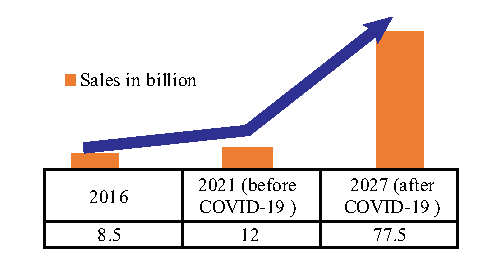
\includegraphics[width=.8\linewidth]{figure/dronesale.eps}
\caption{Predicted sales of drone after and before COVID-19 situation.}
\label{dronesale}
\end{figure}
\section{Challenges}
\label{challengesection}
Drones are becoming more popular in recent days because of technological progress. High-tech systems keep evolving and make flying the drones much easier for us. But more issues emerge with that accessibility. Privacy issues are high on the list of potential drone threats \cite{custers2016flying}. Drones can be used to spy on individuals, to track people persistently, and to collect large scale personal data. The manner drones are being used to gather data, have minimal transparency. Several laws have been enforced to ensure legal protection for privacy. The rules for personal data processing are applied in several national laws, ensuring that the collection and processing of personal data should have a legitimate justification, and is subject to the principles of fair data processing. Therefore, before start using a drone, we need to have a clear vision of drone application.

Drones have several technological limitations. The main ones are limited flight endurance and payload capacity. Most of the common drones nowadays have maximum flight time from 15 to 30 minutes before exchanging or recharging batteries. As flight time of drone has an inverse relationship with payload capacity, one way to increase flight time is to reduce payload. But reducing payload means fewer sensors can be attached to the drone. Besides this, networking is another factor that needs to be handled while working with drones. Operating frequency, data transmission frequencies need to be chosen more carefully. Function in an online network often means the possibility that the network will get hacked. Therefore, the firewall of any drone system should be strong. Another task in the future regarding drones might be the development of the ultimate traffic management system. There is a high probability that drones will become familiar in our daily lives and any traffic control program is being built today, would be out of date.
\section{Conclusion}
\label{conclusionsection}
\textcolor{red}{
In this article, we have presented the latest engineering developments in drone technology and their applications. We have thoroughly investigated the the recent research directions on the network, localization and data management frameworks for drones, especially focusing on the autonomous navigation, safety, signal processing aspects. We then summarized recent trends in application of drones in infrastructure monitoring, object tracking, disaster management, rescue system and supply chain management scenarios. 
}
% We have thoroughly summarized the few recent research work for drone applications, such as autonomous system design, collision avoidance, infrastructure monitoring, object tracking, disaster management, rescue system, data augmentation and compression technique, etc. 
In addition, we have discussed a few benchmark dataset that has been collected by drone and mentioned toolkits that can be used as a data collector. 
Current drone-related research concepts present \textcolor{red}{plethora} of options for pre-processing, post-processing, autonomous operation, analysis, and visual representation with a minimal physical workflow. 
Nonetheless, a lot of issues in this area remain unexplored, 
\textcolor{red}{especially regarding the maintaining the privacy and security of users.}
  Therefore, our belief is that the opportunities and challenges highlighted in this survey would help upcoming researchers, who are aiming to improve drone applications.

%\subsection{Networking}

%\subsection{Computer Vision}
%Object Tracking, Data Augmentation

%\subsection{Hardware platform}
%something related to mechanical
\bibliography{sample}

\end{document}